\documentclass[11pt, oneside]{article}   	
\usepackage[margin=0.5in]{geometry}                		
\evensidemargin=0.25in  
\oddsidemargin=0.25in 
\textwidth=6.25in

\usepackage{fancyhdr}
\pagestyle{fancy}
\fancyhf{}
\fancyhead[R]{\thepage}


\usepackage{graphicx,color}	

%%% color defines
\definecolor{green}{rgb}{0.0, 0.5, 0.0}			
\definecolor{red}{rgb}{1.0, 0.13, 0.32}
\definecolor{blue}{rgb}{0.0, 0.5, 1.0}	
\definecolor{orange}{rgb}{0.93, 0.57, 0.13}
\definecolor{purple}{rgb}{0.6, 0.33, 0.73}
\definecolor{brown}{rgb}{0.44, 0.26, 0.08}
					
\usepackage{amssymb, amsmath, amsfonts, amsthm, multicol}

\newenvironment{myitemize}
{ \begin{itemize}
    \setlength{\itemsep}{0pt}
    \setlength{\parskip}{0pt}
    \setlength{\parsep}{0pt}     }
{ \end{itemize}                  } 

\renewcommand\qedsymbol{$\blacksquare$}

\author{Jordan Greene}

\begin{document}
\newcommand{\modular}[1]{\; \mbox{(mod $#1$)}}
\thispagestyle{empty}

\mbox{}
\setcounter{page}{1}
      
%%%%%%%%%%%%%%%%%%%%%%%%%%%%%%%%%%%%%%%%%%%%%%%%%%%%%%%%%%%%%%%%%%
   	   % Start Document
%%%%%%%%%%%%%%%%%%%%%%%%%%%%%%%%%%%%%%%%%%%%%%%%%%%%%%%%%%%%%%%%%%
\noindent
MPLNet Lidar Site
\hfill Afterpulse / Darkcounts Instructions\\

\noindent\textbf{\LARGE Afterpulse}

\begin{myitemize}
\item Entire procedure takes place in the same hour, starting at the top of the hour
\item Stop collection with the SigmaMPL software just after the hour mark
\begin{myitemize}
\item The \textbf{Stop Collection} button 
\includegraphics[scale=0.3]{stopcollection_button.png} is on the 
	\textbf{Hardware} tab 
\includegraphics[scale=0.3]{hardware_tab.png}
\end{myitemize}
\item Place the cover on the laser
\item With the \textbf{cover on, laser on, shutter on} run collection for approximately 30-35 minutes
\item Stop collection and close completely out of SigmaMPL program
\item Find file created for the time frame and modify the file name to xxx.\textbf{ap}.mpl
\begin{myitemize}
\item File will be located in the data folder and named YYYYMMDDHHMM.mpl
\item Where YYYY is year, MM month, DD day, HH hours, and MM minutes
\item Example: 202205190145.mpl would be renamed to 202205190145.ap.mpl
\item Data Folder Path:\begin{verbatim}C:/Program Files (x86)/SigmaMPL/DATA/\end{verbatim}
\end{myitemize}

\end{myitemize}

\noindent\textbf{\LARGE Dark Counts}

\begin{myitemize}
\item Ensure collection is off from the end of afterpulse procedure (SigmaMPL may still be closed at this point)
\begin{myitemize}
\item The \textbf{Stop Collection} button 
\includegraphics[scale=0.3]{stopcollection_button.png} is on the 
	\textbf{Hardware} tab 
\includegraphics[scale=0.3]{hardware_tab.png}
\end{myitemize}
\item Turn the \textbf{shutter off} on the Photonics controller
\begin{myitemize}
\item This button is located physically on the controller beneath the Lidar
\end{myitemize}
\item Allow the laser to sit for approximately 10 minutes to allow for the residual photons to dissipate
\item Open the SigmaMPL software if not currently open {\begingroup
\setbox0=\hbox{
\includegraphics[scale=0.3]{sigmampl_icon.png}}%
\parbox{\wd0}{\box0}\endgroup}

\item With the \textbf{cover on, laser on, shutter off} run collection for approximately 10 minutes
\begin{myitemize}
\item The \textbf{Start Collection} button is on the \textbf{Hardware} tab 
\includegraphics[scale=0.3]{hardware_tab.png}
\end{myitemize}
\item Stop collection and close completely out of the SigmaMPL program
\item Find file created for the time frame and modify the file name to xxx.\textbf{dc}.mpl
\begin{myitemize}
\item File will be located in the data folder and named YYYYMMDDHHMM.mpl
\item Where YYYY is year, MM month, DD day, HH hours, and MM minutes
\item Example: 202205190145.mpl would be renamed to 202205190145.dc.mpl
\item Data Folder Path:\begin{verbatim}C:/Program Files (x86)/SigmaMPL/DATA/\end{verbatim}
\end{myitemize}
\end{myitemize}

\noindent\textbf{\LARGE Completion}

\begin{myitemize}
\item With \textbf{cover off, laser on, shutter on} restart normal collection at the top of the hour
\item Ensure that data is transferred at 5 minutes after the hour
\end{myitemize}
	
\newpage
\noindent\textbf{\large Notes}\\

\noindent Afterpulse raw data should show a reading at the lowest level (cover on), with no higher altitude counts.\\ 

\noindent Dark counts should have no reading at all due to shutter being closed.\\

\noindent {\begingroup
\setbox0=\hbox{
\includegraphics[scale=0.4]{sigmampl_icon.png}}%
\parbox{\wd0}{\box0}\endgroup} Opens the SigmaMPL program \hfill
{\begingroup
\setbox0=\hbox{
\includegraphics[scale=0.4]{sigma_dir.png}}%
\parbox{\wd0}{\box0}\endgroup} Opens the SigmaMPL directory\\

\noindent If the \textbf{Hardware} tab 
\includegraphics[scale=0.3]{hardware_tab.png} is not open it can be opened from the \textbf{File} menu by selecting \textbf{Real Time Hardware Control}.\\

\begin{center}
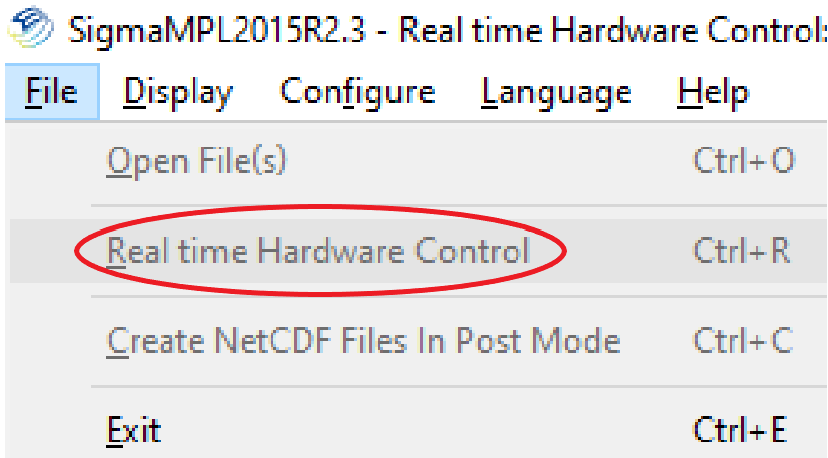
\includegraphics[scale=0.7]{open_hardware.png}
\end{center}


%%%%%%%%%%%%%%%%%%%%%%%%%%%%%%%%%%%%%%%%%%%%%%%%%%%%%%%%%%%%%%%%%%
	% End Document	
%%%%%%%%%%%%%%%%%%%%%%%%%%%%%%%%%%%%%%%%%%%%%%%%%%%%%%%%%%%%%%%%%% 
           
\end{document}  